%%%%%%%%%%%%%%%%%%%%%%%%%%%%%%%%%%%%%%%%
% University/School Laboratory Report
% LaTeX Template
% Version 3.1 (25/3/14)
%
% This template has been downloaded from:
% http://www.LaTeXTemplates.com
%
% Original author:
% Linux and Unix Users Group at Virginia Tech Wiki 
% (https://vtluug.org/wiki/Example_LaTeX_chem_lab_report)
%
% License:
% CC BY-NC-SA 3.0 (http://creativecommons.org/licenses/by-nc-sa/3.0/)
%
%%%%%%%%%%%%%%%%%%%%%%%%%%%%%%%%%%%%%%%%%

%----------------------------------------------------------------------------------------
%	PACKAGES AND DOCUMENT CONFIGURATIONS
%----------------------------------------------------------------------------------------

\documentclass{article}
\usepackage[utf8]{inputenc}
\usepackage[italian]{babel}
\usepackage{appendix}
\usepackage{geometry}
\usepackage[T1]{fontenc}
\usepackage{siunitx} % Provides the \SI{}{} and \si{} command for typesetting SI units
\usepackage{graphicx} % Required for the inclusion of images
\usepackage[numbers]{natbib} % Required to change bibliography style to APA
\usepackage{amsmath} % Required for some math elements 
\usepackage{caption}
\usepackage{tikz}
\usepackage{pdfpages}
\usepackage{url}
\usepackage{hyperref} % Required for href links
\hypersetup{
    colorlinks=true,
    linkcolor=black,
    filecolor=magenta,      
    urlcolor=cyan,
    pdftitle={Simulatore di Sistemi Elettorali in python},
    pdfpagemode=FullScreen,
    }

\usetikzlibrary{arrows,automata, positioning}

\usepackage{import}

\setlength\parindent{0pt} % Removes all indentation from paragraphs

%\renewcommand{\labelenumi}{\alph{enumi}.} % Make numbering in the enumerate environment by letter rather than number (e.g. section 6)

%\usepackage{times} % Uncomment to use the Times New Roman font

%----------------------------------------------------------------------------------------
%	DOCUMENT INFORMATION
%----------------------------------------------------------------------------------------

\title{Simulatore di Sistemi Elettorali in Python} % Title
\author{Mirko Li Veli \\ Alessandro Zito} % Author name
\date{A.A. 2021-22}

\begin{document}
\maketitle % Insert the title, author and date
\begin{center}
\begin{tabular}{l r}
Matricole: & 889700 - 890219\\ % Partner names
Codici Persona: & 10562617 - 10617579\\
Referente progetto: & Gianluca Agosta\\
Referente corso: & Gianluca Palermo % Instructor/supervisor
\end{tabular}
\end{center}

\newpage

\tableofcontents

\newpage


% If you wish to include an abstract, uncomment the lines below
% \begin{abstract}
% Abstract text
% \end{abstract}

%----------------------------------------------------------------------------------------
%	SECTION 1
%----------------------------------------------------------------------------------------




\section{Requisiti e scopo del Progetto}

Il \textit{Progetto di Ingegneria Informatica} (PII abbreviato) è un insegnamento da 5 CFU in cui viene scelto in autonomia dagli studenti uno dei progetti proposti sul \href{https://pii.dei.polimi.it/}{sito del progetto}.
Il progetto da noi selezionato è \textit{Simulatore di Sistemi Elettorali in Python}, ed ha come obiettivo la realizzazione di un simulatore di sistemi elettorali usando come dati in ingresso gli open data del Ministero dell’Interno relativi alle elezioni politiche del 2013 (quando saranno disponibili, anche quelli relativi alle elezioni politiche del 2018). Il nostro lavoro si è incentrato sulla simulazione della legge Binomiale, una legge utilizzata tra il 1998 e il 2013 durante le elezioni del governo in Chile. Abbiamo continuato il lavoro già avviato da altri studenti, che avevano precedentemente creato un framework con il quale è possibile simulare il funzionamento di leggi di questo genere.
Un simulatore di sistemi elettorali può essere utile per molteplici motivi:innanzitutto può essere un buon strumento per scovare casi particolari non trattati per errore dai legislatori; in più, rende facile
studiare come le caratteristiche di queste leggi si riflettono sulla composizione degli organi di governo.


\subsection{La consegna}
Il nostro progetto ha avuto come lavoro principale l’implementazione di una nuova legge elettorale basata sul framework scritto da altri studenti che hanno svolto il medesimo progetto durante gli anni precedenti.
Oltre all'implementazione del sistema di voto binomiale (che verrà presentato nei prossimi capitoli), ci siamo concentrati sulla redazione di una documentazione che amalgami tutte le precedenti e presenti il nuovo sistema di voto, in modo tale da facilitare l'utilizzo del framework per gli studenti futuri.

 
%----------------------------------------------------------------------------------------
%	SECTION 2
%----------------------------------------------------------------------------------------

\section{La Legge Binomiale}
Il sistema binomiale è un sistema di voto utilizzato nelle elezioni legislative del Cile tra il 1989 e il 2013.\newline
Dal punto di vista del sistema elettorale, il sistema binomiale è a tutti gli effetti il metodo D'Hondt con una lista aperta in cui ogni collegio elettorale restituisce due (da cui il nome) rappresentanti al corpo legislativo. Il fatto che in ogni circoscrizione siano eletti solo due candidati risulta nella particolarità in cui è sovra rappresentata la seconda lista di maggioranza. Il suo uso è stato prescritto nella rispettiva legge organica costituzionale durante il regime di Pinochet.\newline
Il sistema binomiale è stato inventato in Polonia negli anni '80 sotto il regime di Wojciech Jaruzelski, al fine di promuovere la stabilità politica nel processo di democratizzazione, mantenendo la preminenza del Partito polacco dei lavoratori uniti contro l'ascesa del movimento di opposizione Solidarność, riconosciuto come un sistema che ha promosso il consenso e la negoziazione tra le parti opposte del governo.

\subsection{Funzionamento}
Il sistema funziona nel modo seguente: partiti e candidati indipendenti si raggruppano in liste o coalizioni, fondamentalmente blocchi elettorali. Ciascuna lista propone fino a due candidati per regione elettorale, provincia o altra unità geografica. \newline I voti vengono conteggiati prima per lista invece che per candidato, e salvo che la lista che ha ottenuto la prima maggioranza abbia il doppio dei voti come seconda maggioranza, ciascuna delle due liste ottiene in carica uno dei propri candidati, quello che ha ottenuto il maggior numero di voti. In altre parole, il sistema binomiale significa fondamentalmente che la prima e la seconda maggioranza hanno una rappresentazione uguale a meno che la prima maggioranza non raddoppi la seconda.\newline Il sistema binomiale agisce per equalizzare la rappresentazione della seconda maggioranza al punto da renderla più o meno uguale, o solo leggermente più piccola, di quella della prima maggioranza. Inoltre, agisce per escludere qualsiasi minoranza dal processo, in pratica generando un sistema bipartitico o bipartitico bloccato in cui è estremamente difficile per uno dei blocchi prendere il sopravvento sull'altro.


%----------------------------------------------------------------------------------------
%	SECTION 3
%----------------------------------------------------------------------------------------

\section{Configurazione}
L'estensione del framework si effettua scrivendo opportuni file Python e Yaml. Oltre a creare un file Python in \textit{src/Commons} con funzioni utili ai calcoli che la legge effettuerà, per ogni legge elettorale è
necessario creare e popolare le seguenti cartelle:

\begin{itemize}
\item\textbf{Classes}: conterrà un file (Python o Yaml) per ogni classe che vogliamo definire. Per definire una classe possiamo farla ereditare da diverse meta-classi già disponibili.
\item  \textbf{Instances}: conterrà un file Yaml per ogni classe definita in Classes. In questo file verranno definite le istanze della classe e alcuni dei loro attributi.
\item \textbf{Data}: conterrà delle sottocartelle, una per ogni classe che deve caricare dati da file csv. Questi file verranno posizionati all'interno delle sottocartelle e il loro nome dovrà corrispondere ad un
attributo della classe.
Per una descrizione più esaustiva di tutte le meta-classi e delle modalità di configurazione si rimanda alla documentazione originale del framework.
\end{itemize}


%----------------------------------------------------------------------------------------
%	SECTION 4
%----------------------------------------------------------------------------------------

\section{Considerazioni iniziali}
Il sistema di voto binomiale è un sistema di voto che non è mai stato applicato per nessuna delle elezioni politiche avvenute in Italia fino ad oggi, abbiamo pertanto riscontrato dei pro e dei contro nella suo implementazione; da una parte si ha avuto una maggiore libertà sul come applicare la legge, d’altra parte la stessa legge è stata limitante su alcuni aspetti e scelte progettuali.


\subsection{Entità politiche}
Come spiegato precedentemente, la Legge Binomiale lavora a livello di coalizioni e singoli individui; essendo i nostri dataset scritti a livello di numero di voti ottenuto da ogni partito, l'unica cosa possibile è poter assegnare i seggi al partito e non al candidato. Non essendo però mai stata applicata questa legge in Italia, abbiamo deciso, di comune accordo con il professore, di assegnare il seggio non al partito, bensì direttamente alla coalizione.

\subsection{Entità geografiche}
Ciascuna lista propone fino a due candidati per regione elettorale, provincia o altra unità geografica. Si è deciso quindi di usare come entità geografica la "provincia", in modo tale da avere un numero congruo di seggi da assegnare, ossia 220. Abbiamo preso in considerazione che la legge fosse applicata dopo la riforma del taglio dei parlamentari, quindi i deputati eletti dovrebbero essere 400. Sempre di comune accordo con il professore, abbiamo deciso che 220 potesse essere un numero adeguato a simulare un andamento ipotetico di come si sarebbe eventualmente riempita la Camera dei Deputati applicando la suddetta Legge.


%----------------------------------------------------------------------------------------
%	SECTION 5
%----------------------------------------------------------------------------------------

\section{Documentazione}
Parte della consegna di questo progetto è stata quella di rendere uniformi ed omogenee le documentazioni scritte per questo progetto, aggiungendo quella relativa al sistema di voto binomiale.
Questo lavoro prevedeva una prima fase di lettura di tutte le documentazioni esistenti che ha richiesto parecchio tempo. Le documentazioni presentavano diverse criticità come file incompleti, file scritti in più lingue, file ridondanti tra le diverse cartelle, pezzi di documentazione ridondanti tra i diversi file.
Il nostro lavoro è consistito nel risolvere, dove possibile, queste criticità.
Sono stati volutamente lasciati dei documenti in inglese che avevano in origine lo scopo di descrivere il contenuto della repository a soggetti esterni che la visitassero.
Il resto dei documenti hanno uno scopo didattico e sono stati tradotti o scritti in italiano allo scopo di dettagliare tutti i contenuti tecnici del progetto, in modo da facilitare la lettura ai professori per la loro valutazione e a futuri studenti interessati a questo progetto.


%----------------------------------------------------------------------------------------
%	SECTION 6
%----------------------------------------------------------------------------------------

\section{Implementazione}

Di seguito presento come ho progettato la mia soluzione per l'estensione del framework. Per le ipotesi che ho dovuto adottate si rimanda alla sezione sull'acquisizione dei dati.
Ho deciso di usare 4 classi:

\begin{itemize}
\item \textbf{Circoscrizione\_Estera}: Circoscrizione che rappresenta i voti espressi fuori l'Italia, divisi per \textit{Europa} e \textit{Resto del Mondo}
\item \textbf{Partito}: per rappresentare i partiti politici e le coalizioni.
\item \textbf{Valle D'Aosta}: rappresenta la Circoscrizione della Valle D'Aosta.
\item \textbf{Province}: rappresenta la nostra entità geografica.
\end{itemize}

e una sola lane uninominale.
\newline \newline


%----------------------------------------------------------------------------------------
%	SECTION 7
%----------------------------------------------------------------------------------------

\section{Acquisizione dei dati}
I dati sono stati acquisiti dal portale Open Data del Ministero dell'Interno; tuttavia questi dati non venivano dati come file \textit{.csv}, ma come file \textit{.txt}. Si è quindi deciso di usare \textbf{Microsoft Excel} come strumento, in particolare la funzione \textit{incolla dati da file di testo} per poi manovrarli con le tabelle pivot e far uscire un file \textit{.csv} con i campi necessari per essere utilizzato.\newline \newline
Le province e i partiti invece sono stati isolati tramite un breve script fatto in Javascript per velocizzare la scrittura dei file contenuti nella cartella Instances.


%----------------------------------------------------------------------------------------
%	SECTION 8
%----------------------------------------------------------------------------------------

\newpage
\section{Risultati}

Qui di seguito è mostrata la composizione della Camera in seguito alla mia simulazione delle elezioni del 2013 con la legge Binomiale.

\begin{figure}[h]
    \centering
    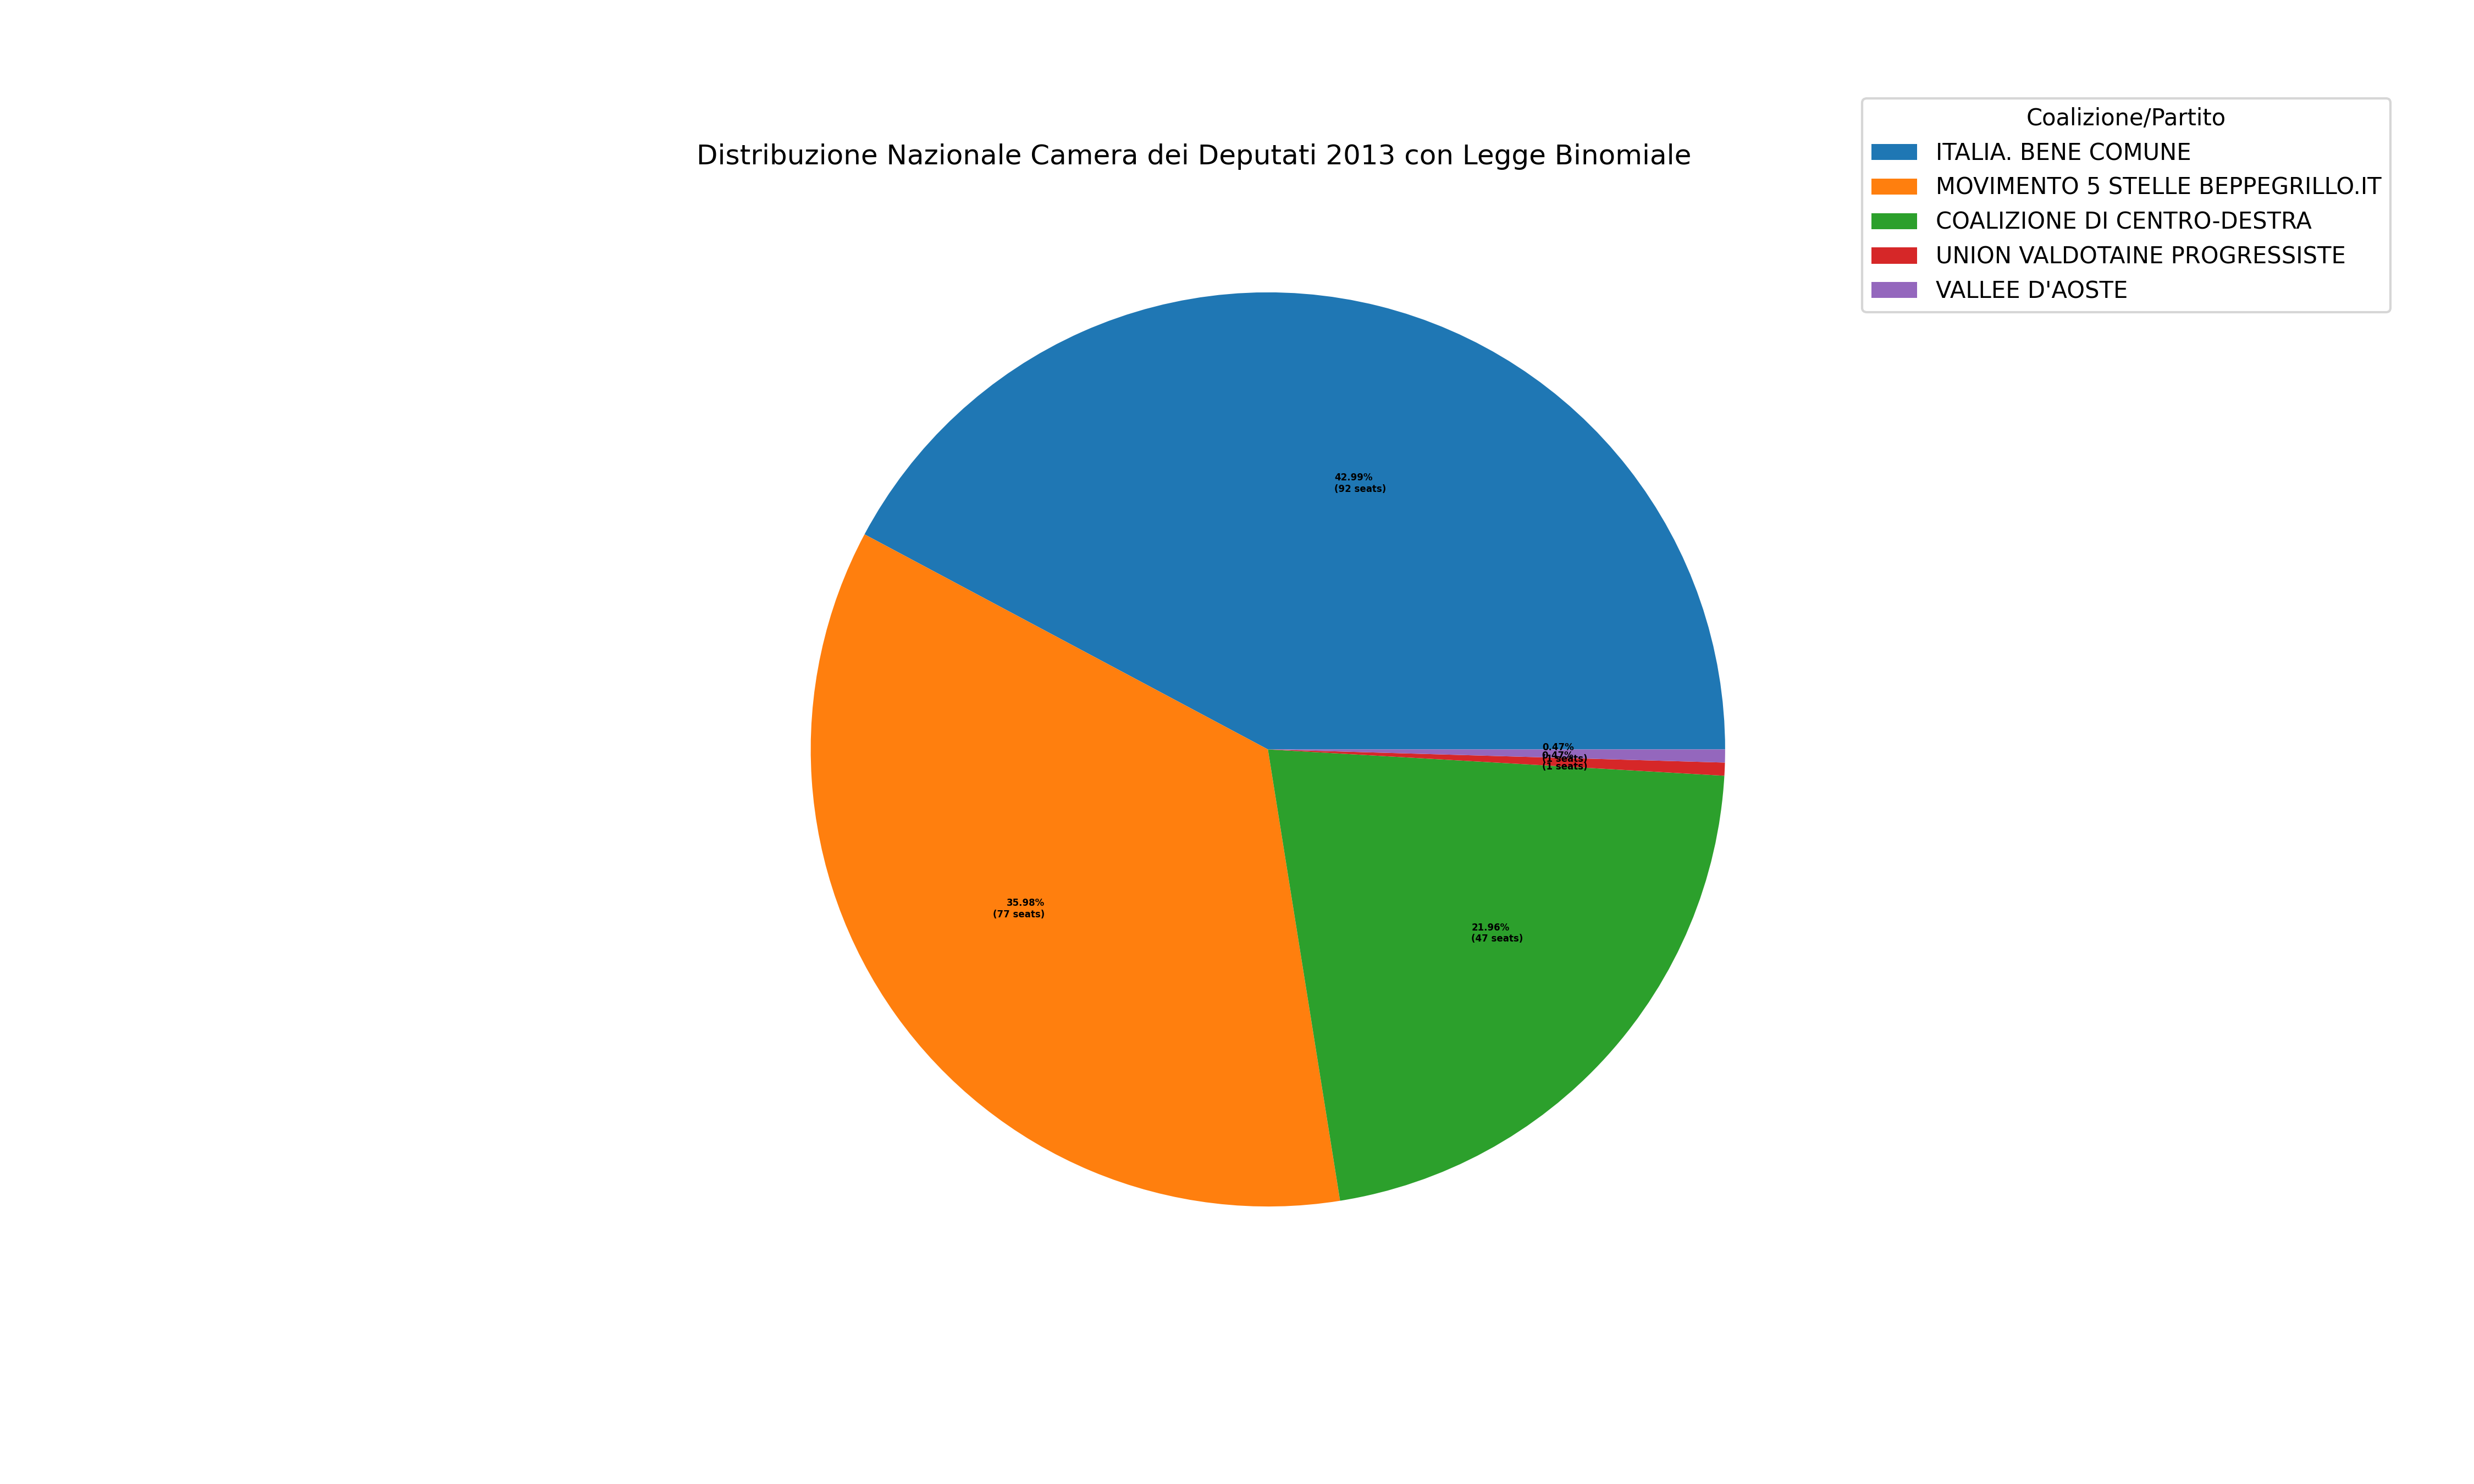
\includegraphics[scale=0.45]{binomiale.png}
    \caption{Risultati con simulazione della "Legge Binomiale"}
    \label{fig:binomiale}
\end{figure}

\newpage

\begin{figure}[h!]
    \hbox{\hspace{-8cm}
    \includegraphics[scale=0.65]{binomiale_plt.png}}
    \caption{Grafico dei risultati generato con matplotlib.plt}
    \label{fig:binomiale_plt}
\end{figure}

\newpage
Notiamo come la legge ha creato tre grosse coalizioni, con differenze non eccessive, limitando a un solo seggio gli altri partiti. È questo l'obiettivo della legge Binomiale, far in modo che non ci sia una coalizione con una maggioranza assoluta.


%----------------------------------------------------------------------------------------
%	SECTION 9
%----------------------------------------------------------------------------------------

\section{Conclusioni}
Il progetto si è stato stimolante ed impegnativo sotto diversi aspetti poiché ci ha permesso di coniugare il nostro interesse per la politica (dandoci la possibilità di approfondire leggi, consultare dati ufficiali e testi originali) con la nostra passione per l’informatica e la programmazione.
Per poter utilizzare al meglio il framework già esistente è stato fatto un grande lavoro di reverse engineering, che si è dimostrata essere la vera difficoltà del progetto. Abbiamo pertanto rilavorato sulle documentazioni già esistenti, creando ordine e completando laddove fosse possibile i pezzi mancanti, aggiungendo ciò che concerne quanto da noi implementato.
Riguardo ai risultati ottenuti, abbiamo fatto delle considerazioni ritenendo che la legge binomiale svantaggi molto la coalizione con più voti in quanto non ottiene seggi in modo proporzionale ai voti ottenuti, come accadrebbe invece con una legge come il Porcellum.
Questa legge infatti è stata considerata dalla maggior parte degli analisti come il principale freno costituzionale che ha impedito il completamento della transizione cilena alla democrazia.
\end{document}
